%%%%%%%%%%%%%%%%%%%%%%%%%%%%%%%%%%%%%%%%%
% Simple Sectioned Essay Template
% LaTeX Template
%
% This template has been downloaded from:
% http://www.latextemplates.com
%
% Note:
% The \lipsum[#] commands throughout this template generate dummy text
% to fill the template out. These commands should all be removed when 
% writing essay content.
%
%%%%%%%%%%%%%%%%%%%%%%%%%%%%%%%%%%%%%%%%%

%----------------------------------------------------------------------------------------
%	PACKAGES AND OTHER DOCUMENT CONFIGURATIONS
%----------------------------------------------------------------------------------------

\documentclass[12pt]{article} % Default font size is 12pt, it can be changed here

\usepackage{geometry} % Required to change the page size to A4
\geometry{a4paper} % Set the page size to be A4 as opposed to the default US Letter

\usepackage{graphicx} % Required for including pictures

\usepackage{float} % Allows putting an [H] in \begin{figure} to specify the exact location of the figure
\usepackage{wrapfig} % Allows in-line images such as the example fish picture

% \usepackage{lipsum} % Used for inserting dummy 'Lorem ipsum' text into the template

\linespread{1.2} % Line spacing

%\setlength\parindent{0pt} % Uncomment to remove all indentation from paragraphs

\graphicspath{{img/}} % Specifies the directory where pictures are stored

\begin{document}

%----------------------------------------------------------------------------------------
%	TITLE PAGE
%----------------------------------------------------------------------------------------

\begin{titlepage}

\newcommand{\HRule}{\rule{\linewidth}{0.5mm}} % Defines a new command for the horizontal lines, change thickness here

\center % Center everything on the page

\textsc{\LARGE Wheaton College (MA)}\\[1.5cm] % Name of your university/college
\textsc{\Large COMP-401}\\[0.5cm] % Major heading such as course name
\textsc{\large Senior Seminar}\\[0.5cm] % Minor heading such as course title

\HRule \\[0.4cm]
{ \huge \bfseries Why AGI Is Not Necessarily Imminent}\\[0.4cm] % Title of your document
\HRule \\[1.5cm]

\begin{minipage}{0.4\textwidth}
\begin{flushleft} \large
\emph{Author:}\\
Bryan \textsc{Jensen} % Your name
\end{flushleft}
\end{minipage}
~
\begin{minipage}{0.4\textwidth}
\begin{flushright} \large
\emph{Professor:} \\
Tom \textsc{Armstrong} % Supervisor's Name
\end{flushright}
\end{minipage}\\[4cm]

{\large \today}\\[3cm] % Date, change the \today to a set date if you want to be precise

%\includegraphics{Logo}\\[1cm] % Include a department/university logo - this will require the graphicx package

\vfill % Fill the rest of the page with whitespace

\end{titlepage}

%----------------------------------------------------------------------------------------
%	TABLE OF CONTENTS
%----------------------------------------------------------------------------------------

\tableofcontents % Include a table of contents

\newpage % Begins the essay on a new page instead of on the same page as the table of contents 


% \begin{figure}[H] % Example image
% \center{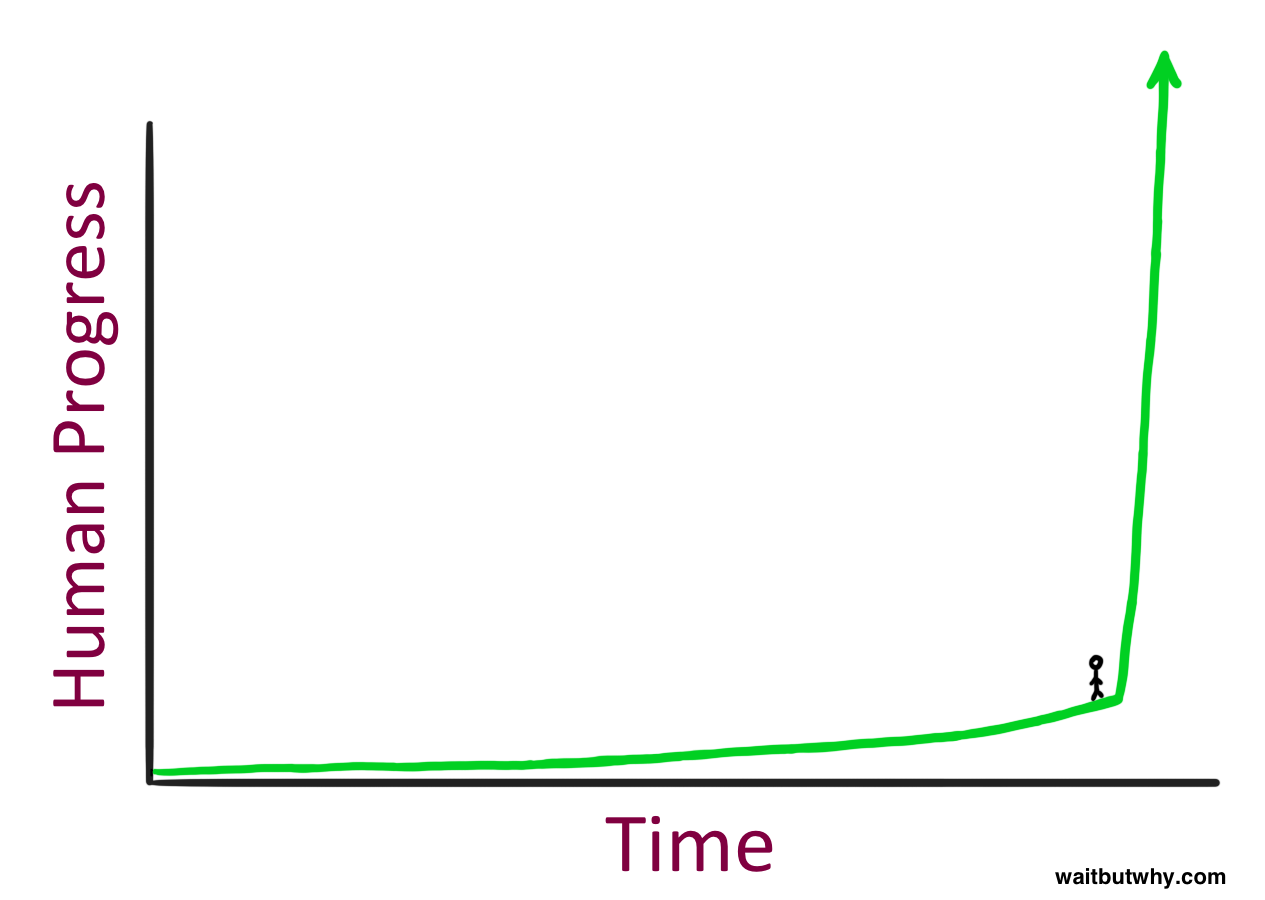
\includegraphics[width=0.5\linewidth]{ontheedge}}
% \caption{Example image.}
% \label{fig:speciation}
% \end{figure}



% \begin{wrapfigure}{l}{0.4\textwidth} % Inline image example
%   \begin{center}
%     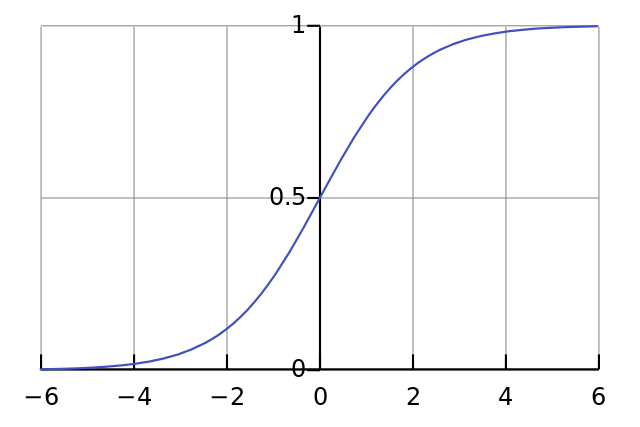
\includegraphics[width=0.38\textwidth]{logisticcurve}
%   \end{center}
%   \caption{Fish}
% \end{wrapfigure}



% \begin{description} % Numbered list example

% \item[First] \hfill \\
% % \lipsum[9] % Dummy text

% \item[Second] \hfill \\
% % \lipsum[10] % Dummy text

% \item[Third] \hfill \\
% % \lipsum[11] % Dummy text

% \end{description} 



% Example citation \cite{Figueredo:2009dg}.



% \bibitem[Figueredo and Wolf, 2009]{Figueredo:2009dg}
% Figueredo, A.~J. and Wolf, P. S.~A. (2009).
% \newblock Assortative pairing and life history strategy - a cross-cultural
%   study.
% \newblock {\em Human Nature}, 20:317--330.

%----------------------------------------------------------------------------------------
%	INTRODUCTION
%----------------------------------------------------------------------------------------

\section{Introduction} % Major section

Artificial Intelligence (AI) has been in the news quite a lot lately, in a different way than ever before. Big names in technology and science have been voicing their concerns in interviews and over Twitter, people such as Elon Musk (the CEO of Tesla Motors, SpaceX and of PayPal fame) and Stephen Hawking (the closest thing to a celebrity physicist since Einstein). Note that these guys are widely considered among the smartest in the world, despite none of them being directly related to AI research. Their concerns fall along the lines of: what our potential new robot overlords may mean for the future of the human race, whether the human race would survive such an event, and just how imminent this ``threat'' is in our immediate future.

The main reason for this recent concern is recent arrival estimates of an event, often referred to as ``The Singularity,'' have placed this event within the next few decades, and the vast majority of AI experts agree that it will certainly happen within our lifetimes. This term \textit{singularity} in general is used to refer to the moment where a function goes to infinity, such as the level of matter density at the center of a black hole. In the field of AI, this \textit{singularity} is used to refer to the moment when progress, specifically in technology, starts to accelerate to the extent where to us it appears to be infinitely fast.

The main expected cause for this is the nature of artificial intelligence. It is believed that Artificial Intelligence has the unique ability to build on itself, producing an exponential growth in its ability to solve problems, which will eventually lead to a increase in power so steep that, to us as humans, it may as well be infinite.

Part of what will feed into AI's ability to produce this exponential growth is the observed exponential growth in computing technology that has taken place over the past few decades. This is most often quoted as ``Moore's Law,'' which states that the number of transistors per square inch on consumer-grade processors would double every 18 months. There are similar laws that deal with the actual speed of processors, the computing power of those processors, and more; all values which are closely related but not identical. Note, the original Moore's Law number was 12 months, and lately seems to be increasing to numbers beyond 18, but as this is still a large increase in computing power every year, it could still allow for huge advances in what's possible.

%----------------------------------------------------------------------------------------
%	Artificial Intelligence
%----------------------------------------------------------------------------------------

\section{Artificial Intelligence} % Major section

Since the singularity is based on an amount of progress made possible by artificial intelligence, it makes sense to examine just what that is.

%------------------------------------------------

\subsection{Quick Overview} % Sub-section

Since the very early days of Computer Science, the ideal of artificial intelligence has always been to match the human brain, to be able to do everything a human can do as well or better. However, there is a large subsection of the field of AI research that doesn't make an attempt to rival the human brain in its general abilities, but rather focuses in on a specific task that is not as well understood and masters that. Since this can blur the line between AI and general algorithms, there appears this phenomenon that a task is described as a form of AI until it is solved and understood, and promptly stops being AI. We'll expand upon this idea later on.

%------------------------------------------------

\subsection{AI in Popular Culture}

By far the most commonly known form of AI is the kind of AI that finds its way into movies, from a larger series such as The Matrix to a newer entry such as Her. This tends to be, as you would expect, a romanticized version of AI, more along the lines of what was originally envisioned as a rival to human intelligence. Also, in the movies most often the AI is embodied in a robot, but as it happens the physical machine that makes the ``robot'' ends up just being a container for the AI, just as our bodies could be considered containers for our brains.

%------------------------------------------------

\subsection{AI in the ``Real World''}

AI research currently tends more towards simplification of the given problem rather than generalization of the technique. What this means is that they take a problem that is viewed as ``hard,'' such as the game of chess, and break it down into solvable, computable chunks. Often this ends up reducing the given problem into a tree, graph or other searchable space, against which we have many well developed tools and algorithms we can leverage.

Another form is a rule-based structure that matches situations with solutions for that situation. This is popular in video gaming, where events can trigger reactions in the AI, intended to address that event to the furthering the AI's goals. For example, a ``bot'' in a computer game may, when presented with a human player with very little remaining health, may employ a tactic to play aggressively and kill the human player, thus completing the corresponding goal pre-programmed into the ``bot.''

%------------------------------------------------

\subsection{What I consider Artificial \textit{Intelligence}}

My definition of AI stresses the \textit{intelligence} half of the term, and encompasses a suite of algorithms referred to as ``genetic algorithms.'' The central concept behind these algorithms is to mimic evolution and thereby learn how to solve a problem starting from complete ignorance and eventually, in theory, becoming a master. The key to these algorithms is that they themselves learn how to solve the problem they're designed for, and do not rely on the knowledge of the programmer embedded in their code.

%------------------------------------------------

\subsection{Real Examples of AI}

There are numerous examples of AI in the world at the moment. For a short while, the most popular of these was DeepBlue, the computer built solely to win chess against the world grand master, a task which it accomplished. Another famous example is Watson, designed by IBM to be capable of beating the world's best players at the TV Show Game \textit{Jeopardy!}, which it managed to do handily to a large audience. A final example, one less well known but likely recognizable, is an attempt by Google to design a system to recognize text in pictures, a system which was actually capable of breaking the spambot-filter systems throughout the internet, known as ``captcha'' or ``reCaptcha''. These are all examples of ``Artificial Narrow Intelligence,'' by far the most common type of AI in the world today.

%----------------------------------------------------------------------------------------
%   Progression of AI
%----------------------------------------------------------------------------------------

\section{Progression of AI}

If Artificial Intelligence is to lead towards something, that implies progression. There is a really interesting progression predicted for the field of AI, with some really scary implications. It starts where we are now, with Artificial Narrow Intelligence (ANI), and concludes with something we have \textit{defined} to be that which we can't understand (interesting), Artificial Super Intelligence (ASI).

%------------------------------------------------

\subsection{Artificial Narrow Intelligence} % Sub-section

ANI covers \textit{everything} in the world of practical AI in the world today. Also called \textit{Weak AI}, it does one job, perhaps very well, and it does nothing else. Watson is an impressive feat of programming and technology, but it only does what it does; attempt to use it to play a video game, and it will have no concept of what that means.

%------------------------------------------------

\subsection{Artificial General Intelligence} % Sub-section

AGI, often called \textit{Strong AI} covers the entire concept of a form of AI that can compete with humans in every area, from chess to talking to figuring out the concept of making a cup of coffee. This has been the goal of AI research since its inception, and is expected to be the invention that sparks the singularity.

%------------------------------------------------

\subsection{Artificial Super Intelligence} % Sub-section

This is a realm of intelligence that is incomprehensible to humans. An ASI entity trying to explain what it knows to us, would be analogous to humans trying to explain society and our more advanced concepts to a dog. There is simply no understanding for the recipient. It is expected that once we hit AGI, that achievement can be leveraged to improve itself, and it won't be long after that that we find ourselves in ``possession'' of an ASI.

%----------------------------------------------------------------------------------------
%	Singularity
%----------------------------------------------------------------------------------------

\section{``The Singularity''}

\begin{wrapfigure}{l}{0.40\textwidth} % Inline image example
  \begin{center}
    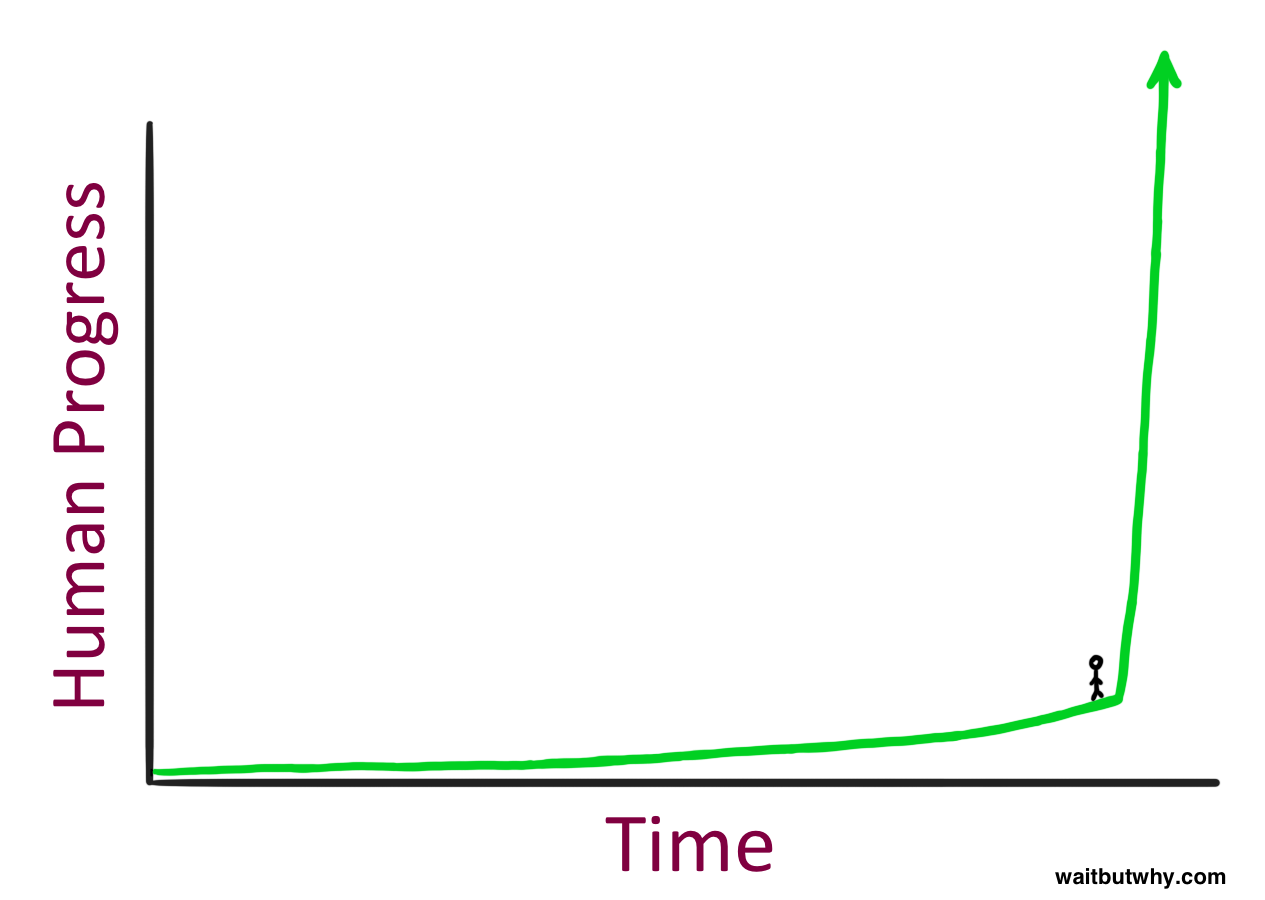
\includegraphics[width=0.38\textwidth]{ontheedge}
  \end{center}
  \caption{Sudden Exponential Growth}
\end{wrapfigure}

``The Singularity,'' if you will recall, is the moment where the rate of increase of intelligence may as well be infinite. This is expected to happen immediately following the first instance of AGI - once that happens, the AI can begin the process of improving itself as well as a human could. Since that process inherently feeds back into itself, we will start seeing exponential growth almost immediately.

Imagine that we are standing, in time, at the position of the stick figure. In the near future we develop AGI, and that AGI starts improving itself. The amount of intelligence of the smartest organism on earth (previously humans, now an AGI), will skyrocket.

Many smart people, including Elon Musk and Stephen Hawking, have raised very accurate issues about the amount of power that an entity that is vastly superior to humans will inherently have. We have no reason to expect that this new intelligence, which malicious or benign, will at any moment wipe us out for one reason or another. There are countless scenarios that involve no intent on the side of the perpetrator, but still result in the death and extinction of the victim. Just one of these scenarios need occur for the human race to be wiped out by our new creation.


%----------------------------------------------------------------------------------------
%   Moore's Law
%----------------------------------------------------------------------------------------

\section{Moore's Law}

With how scary that eventuality is, it is no surprise that it is what gets the majority of the focus when talking about advances in technology and artificial intelligence. However, the vast majority of talk and predictions about the upcoming singularity base its inevitability on the steady and massive increases in technological power at our disposal. The thinking is, if we develop a powerful enough computer, then our algorithm doesn't have to be efficient to be smart, and by increasing that power we can eventually manufacture a system smarter than we are.

The problem with this scenario is its reliance on Moore's Law, a law that has held true for half a century of computational advances, so why would it come into question now? The issue is that, while Moore's Law has held for this long, it has slowed over time and there is no reason to believe it will provide the driving power for the creation of AGI.

%------------------------------------------------

\subsection{What is Moore's Law?} % Sub-section

Moore's Law, at its essence, dictates that computing power increases at an exponential rate with regards to time. Its official form states that ``the number of transistors per square inch on consumer-grade processors will double every 18 months.'' The original number quoted by Gordan Moore, a co-founder of Intel, was 12 months, but he has since endorsed the above version stating the longer period.

%------------------------------------------------

\subsection{What's Wrong with Moore's Law?} % Sub-section

The law was originally stated in 1965, and since then the law has held true - for the most part. Part of the reason this has been true is that the law became a self-fulfilling prophecy; it became the industry goal, and hence spawned a second, sister Moore's Law (also known as Rock's Law): the cost of an Research \& Development lab would also increase exponentially over time. With money being a finite resource, it is understandable why both of these could not continue forever.

%------------------------------------------------

\subsection{Moore's Law Overcoming Hurdles} % Sub-section

Despite the above issues with Moore's Law, as well as other issues (not the least of which being the fundamental boundary of the size of an atom restricting the very size of transistors), Moore's Law has overcome quite a few hurdles since its inception, and many seem undaunted about its ability to continue to improve our computational power.

One such hurdle was in 2005, and was quickly overcome by the shift from single-core processors to the current paradigm of multi-core. While this is not a strict improvement, it allowed for computational power to continue its steady climb. Other industry breakthroughs also allowed Moore's Law to continue in defiance of those who heralded its death.

Each of these advances, however, seems to be a stopgap measure and not an indication that Moore's Law will continue forever. There is no getting around the fact that one (as we currently understand it) cannot go beyond the level of an atom in size. But Moore's Law does not have to continue forever.

%------------------------------------------------

\subsection{AGI or ASI can solve it!} % Sub-section

Assuming we can continue the march of Moore's Law long enough to develop full AGI, the common thinking is that the new entity will be smart enough to help develop its own advances in computing power, and solve that issue while simultaneously improving itself in other ways. There is utter faith that if we manage to develop full ASI, then it will be able to solve all such problems, as its ability to understand the nature of things and the universe will be so far beyond ours that we need not understand its solution, just that it works.

%----------------------------------------------------------------------------------------
%   Inevitable Progress
%----------------------------------------------------------------------------------------

\section{Inevitable Progress} % Major section

% Inline image
\begin{wrapfigure}{l}{0.50\textwidth}
  \begin{center}
    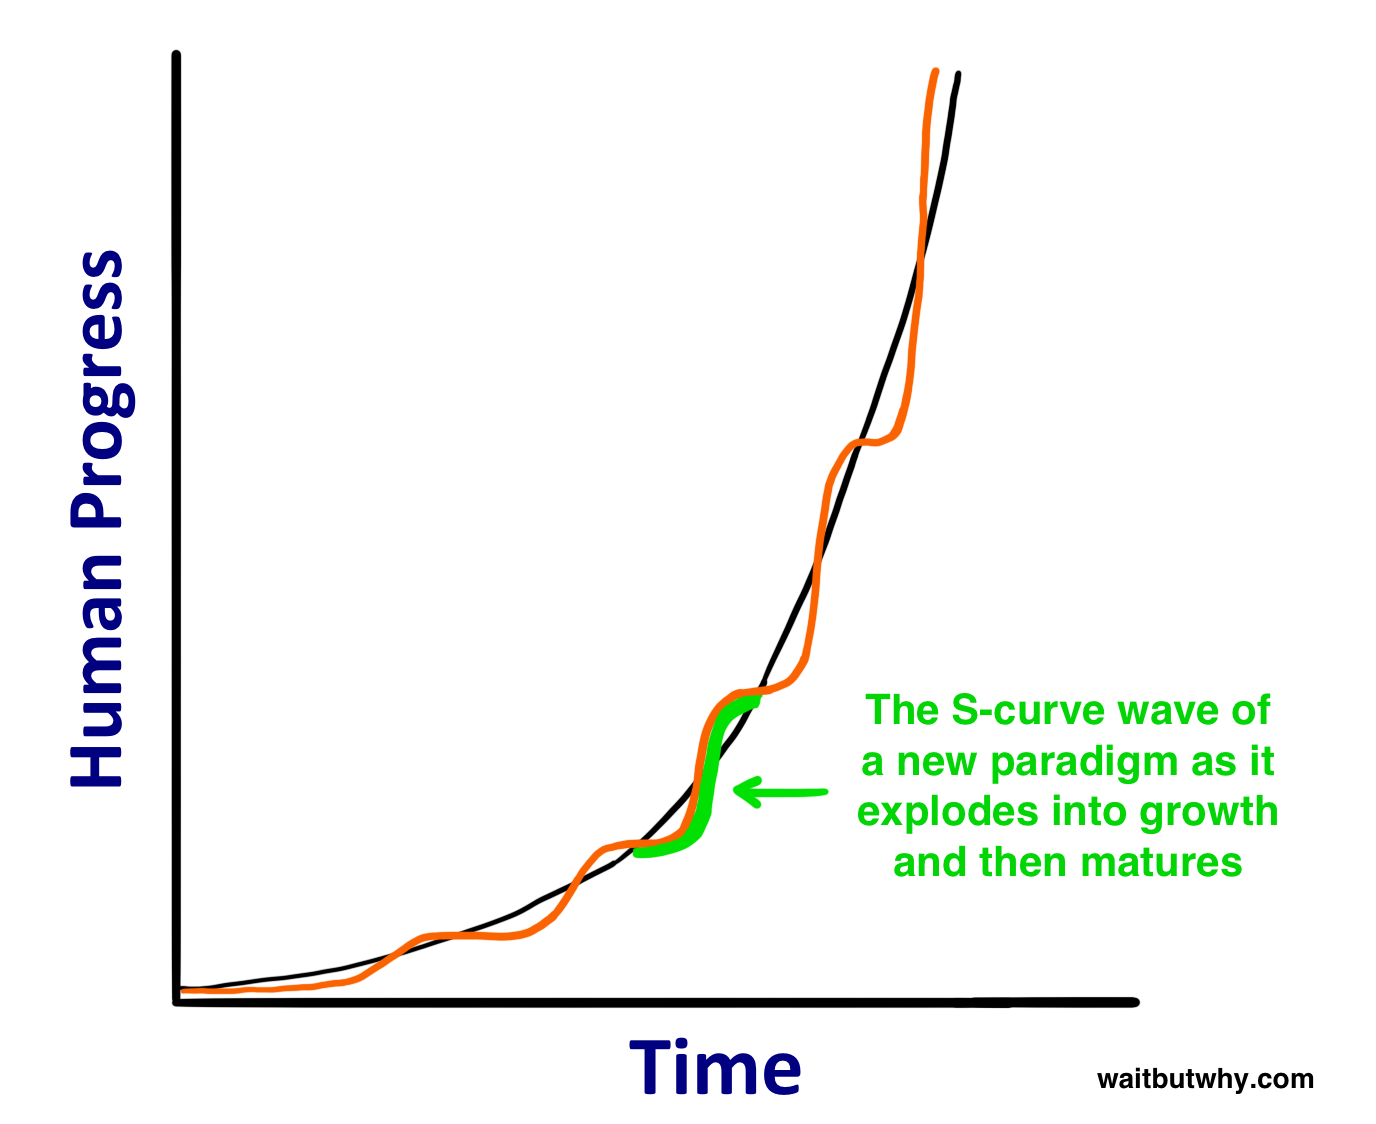
\includegraphics[width=0.48\textwidth]{curvyexponential}
  \end{center}
  \caption{Inexorable Progress}
\end{wrapfigure}

There is one main point that pretty much everyone quotes as the reason that we must, some time in the near future, develop AGI: human progress is exponential. It may slow for a short time, but it eventually makes such leaps and bounds that modern day society is unrecognizable even 200 years ago. To understand this, consider this hypothetical time travel: Take a man from 1600 and place him in 1800. This experience may be eye-opening, but it will be much less traumatizing and confusing than taking a man from 1800 and dumping him in modern day society as of 2015. We have developed so much in the way of technology in the past century alone, that for it to be comparable, you would need to take a man from much farther back - perhaps to before the birth of cities and cultures and art and technology and math - and drop him in 1800, for him to feel the same way as the 1800 man in 2015.

And the main point they like to emphasize is how ridiculous the nay-sayers look with the 20-20 hindsight of history. Progress marches on, great inventions happen every decade, every year, every month. We must embrace and expect the change, in order to properly plan for it.

But the one main issue with this line of argument is our continual inability to correctly predict the future. There are stereotypical examples of inventions that people of the 1960's expected would be commonplace by the year 2000, namely space travel, flying cars and automatic doors. Only the last of these has been achieved to a household level. This is just one example showing that, even though we know progress will happen and happen quickly, we never know what form it will take.

So my argument becomes not that we as a race won't progress, and that we won't develop something of the same magnitude as ASI, but rather that we simply don't know what that innovation will look like. 

%----------------------------------------------------------------------------------------
%	Conclusion
%----------------------------------------------------------------------------------------

\section{Conclusion} % Major section

I will not say for certain that AGI and ASI are impossible parts of our (very near) future. But I also do not wish to claim that, for the first time in recorded history, we can attempt to see even 10 years into the future, for those 10 years may be more different from today than 1915 is from 2015. But it is just as possible that 2025 may come and go without much change from our current situation.

I will not, however, believe claims stating that AGI is imminent when those claims are based on Moore's Law. While Moore's Law is projected to hold out for another possible two decades, even today its progress is slowing, and it cannot be relied upon as the driving force behind \textit{true} artificial intelligence. I will believe that within my lifetime we will see many more changes that dramatically alter society, quite likely more than in the past millennium. But we have no way of knowing what form those changes will take, or even if they will be instigated by technology as we understand it today.

Artificial Narrow Intelligence is a powerful force in our world today. Artificial General Intelligence has the power to easily change our world. Artificial Super Intelligence has the power to easily end our world. But none of it is guaranteed to happen as the experts seem convinced is imminent.

%----------------------------------------------------------------------------------------
%	BIBLIOGRAPHY
%----------------------------------------------------------------------------------------

\begin{thebibliography}{99} % Bibliography - this is intentionally simple in this template
 
\end{thebibliography}

%----------------------------------------------------------------------------------------

\end{document}